\section{Results and interpretation}
\label{sect:stat}
Event data yields and background predictions for the four signal regions are summarized in Table~\ref{tbl:yieldSysSummary}.
There is no excess of events over the SM expectation.  We interpret our results in the context
of a simplified model of chargino pair-production and decay, which corresponds to the left
diagram in Fig.~\ref{fig:Productions}. This is a simplified model when a pair of \chione 
are produced and decay exclusively to the shown final states which contain two $\tau$, two $\nu_{\tau}$ and two \PSGczDo.
The mediators in the decay of \chione can be either \sTau or $\sNu_{\tau}$. All  \sTau and $\sNu_{\tau}$ 
are produced  on-shell. They have equal masses which is the mean value of the masses of the \chione   and \PSGczDo.
The two distinct decay chains in the left diagram of Fig.~\ref{fig:Productions} are assumed to have equal branching ratios, which is 50\%.

\begin{table}[!htb]
\begin{center}
%\begin{tiny}
\caption{Data yields and background predictions with uncertainties in the four signal regions of the search. 
%The first two lines are based on Monte Carlo simulation, when for the first row, a validation against data is also done. 
%The last two rows are data driven, but the ``Fake'' for the \tauTau channel is not completely data driven.
%The uncertainties are systematic, unless when there are two parts, the first part is statistics.
The uncertainties are reported in two parts, the statistical and systematic uncertainties, respectively. 
%For \wjets in \tauTau channel, the full uncertainty is
%reported and considered as systematic for ``SM Total''.
The main backgrounds (\wjets and QCD multijet) are derived from data as described in Section~\ref{sect:bkg},
The abbreviation ``VV'' refers to diboson events.
}
\begin{tabular}{|c|c|c|c|c|}
\hline
	           & \eTau & \muTau & \tauTau \binone & \tauTau \bintwo \\
\hline
 Z+jets            & 0.19 $\pm$ 0.04 $\pm$ 0.03 & 0.25 $\pm$ 0.06  $\pm$ 0.04  &  0.56 $\pm$ 0.07 $\pm$ 0.12 & 0.81 $\pm$ 0.56 $\pm$ 0.18  \\
\ttbar, VV, hX  & 0.03 $\pm$ 0.03 $\pm$ 0.02 & 0.19 $\pm$ 0.09  $\pm$ 0.09  &  0.19 $\pm$ 0.03 $\pm$ 0.09 & 0.75 $\pm$ 0.35 $\pm$ 0.38  \\
\wjets             & 3.30 $\pm$ 3.35 $\pm$ 0.56 & 8.15 $\pm$ 4.59  $\pm$ 1.53  &  0.70 $\pm$ 0.21 $\pm$ 0.55 & 4.36 $\pm$ 1.05 $\pm$ 1.63  \\
QCD multijet       &             -              &            -                 &  0.13 $\pm$ 0.06 $\pm$ 0.21 & 1.15 $\pm$ 0.39 $\pm$ 0.74  \\
\hline
SM total           & 3.52 $\pm$ 3.35 $\pm$ 0.56 & 8.59 $\pm$ 4.59  $\pm$ 1.53  &  1.58 $\pm$ 0.23 $\pm$ 0.61 & 7.07 $\pm$ 1.30 $\pm$ 1.84  \\
\hline
\hline
Observed           &               3            &                5             &             1               & 2     \\  
\hline
\end{tabular}
\label{tbl:yieldSysSummary}
\end{center}
\end{table}


Combining all four signal regions,
the search rules out \chione of mass up to 410 \GeV and  $\PSGczDo$ of mass up to 100 \GeV,
see Fig.~\ref{fig:limit_final}. 
%%%%%%%%%%
\begin{linenomath}
\begin{figure}[h]
\centering
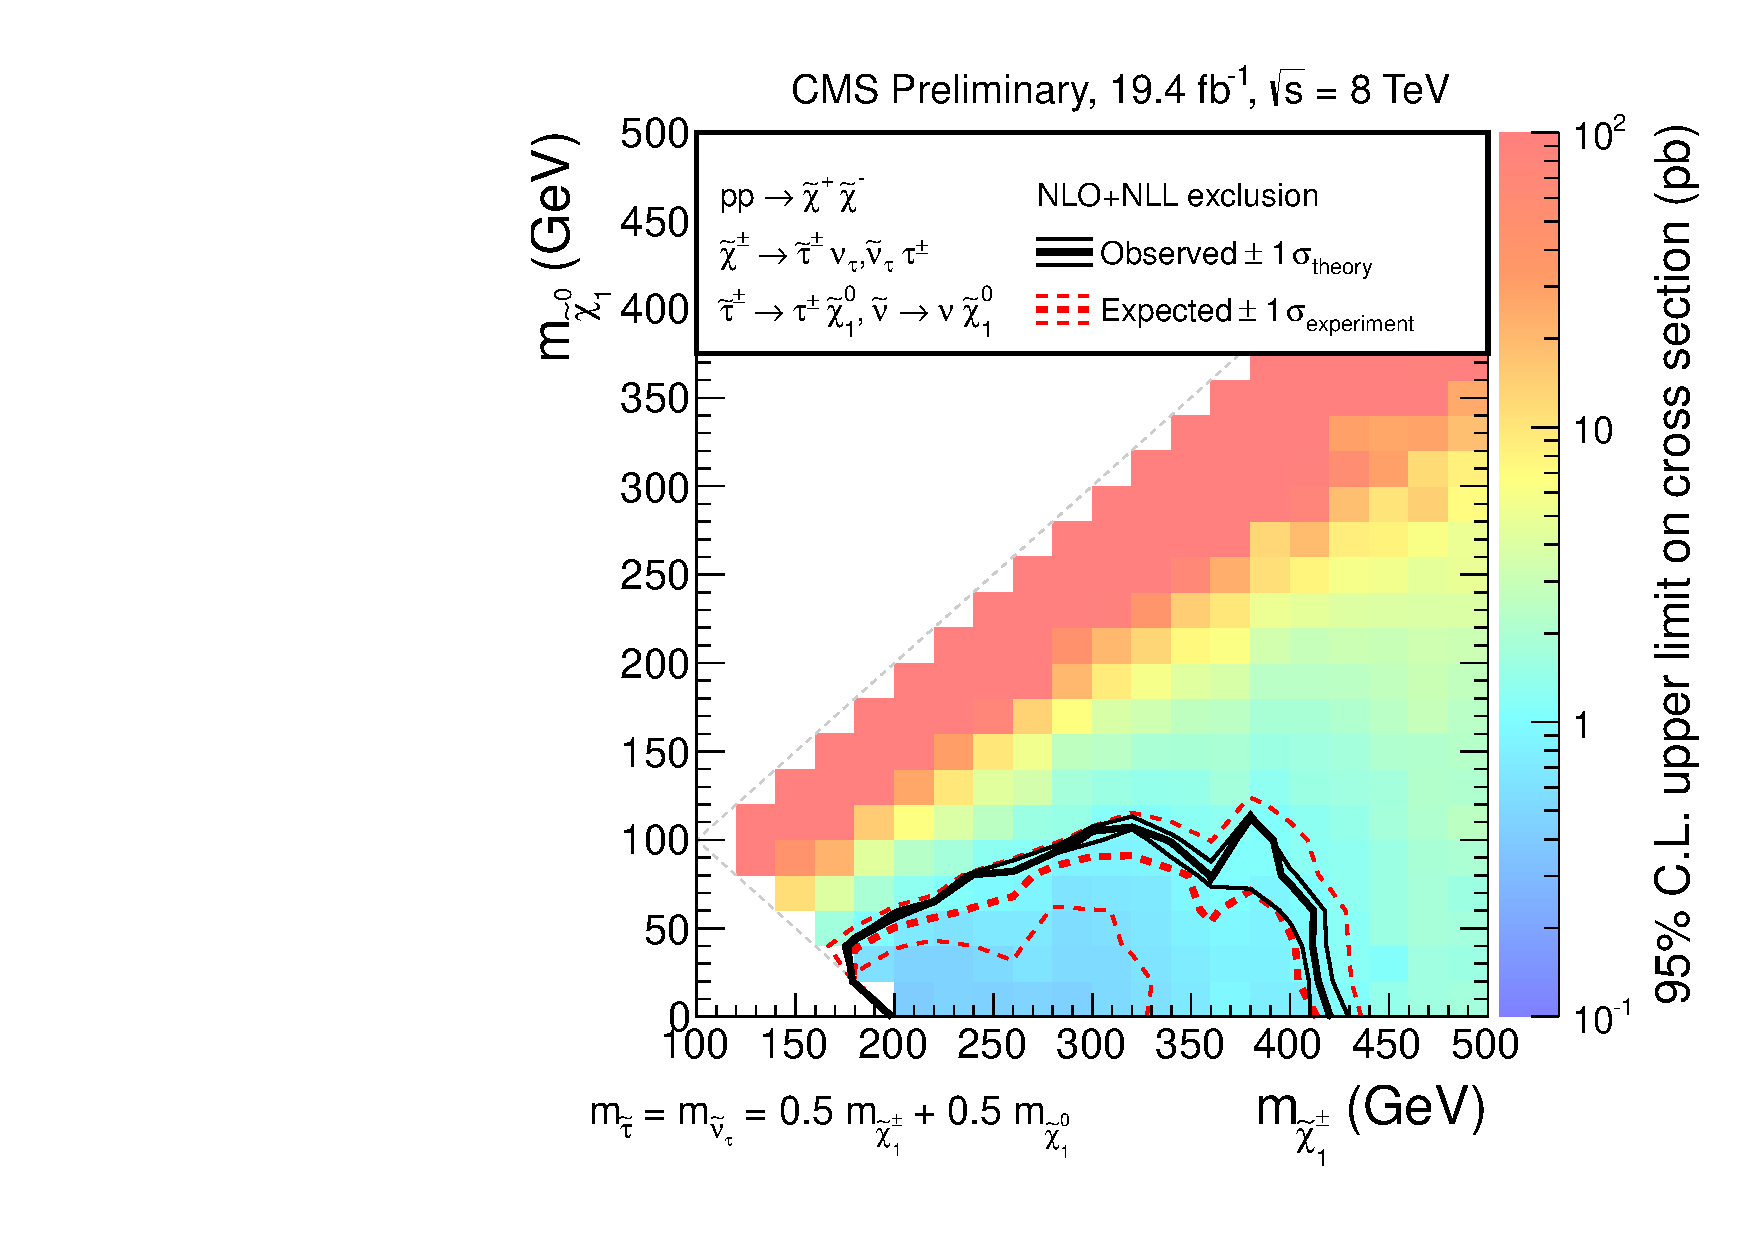
\includegraphics[width=0.7\textwidth,keepaspectratio=true]{StatisticsFig/Exclusion4Bins.pdf}
\caption{Expected and observed exclusion power in terms of Simplified Models
with the total dataset of 2012. 
%Backgrounds are predicted using Monte-Carlo simulations and a rough estimate of systematic uncertainties equal $10\%$ is taken into account.
}
\label{fig:limit_final}
\end{figure}
\end{linenomath}
%%%%%%%%%%
This is conducted using a modified frequentist approach, namely CLs method \cite{read:CLs} to 
exclude the signal points at 95\% Confidence Level.
The \sTau searches in the LEP experiments \cite{lepsusy} have excluded the masses below 95 \GeV. In Fig.~\ref{fig:limit_final}, 
this region corresponds to the triangle in bottom-left corner.% is shown by the line labeled as $m_{\sTau} < 95 GeV$. 
The diagonal line denotes the boundary for $m_{\chione} = m_{\tau} + m_{LSP}$, which is the kinemtical boundary of the search.
The expected limits and their one standard deviations introduced by the experimental 
uncertainties are shown with the red solid and dashed lines, respectively. The observed limits are shown with the black solid lines, the one 
standard deviations are shown with narrower black lines. The theoretical cross sections are moved up and down by one one standard deviation to 
find the narrow lines.
The signal cross sections in NLO + next-to-the-leading-logarithm (NLL) order in $\alpha_s$ are used to make the exclusion limits.
In the whole region, the observed limits lie closer than one standard deviation from the expected limits.  

The results of the \tauTau channels are interpreted to set limit on the $\tilde{\tau}\tilde{\tau}$ production, which corresponds to the right diagram in Fig.~\ref{fig:Productions}. In this simplified model, two $\tilde{\tau}$ are directly produced from the $pp$ collision and decay instantly into two $\tau$ and two \PSGczDo. As the cross section of direct production of sleptons is lower,
\begin{linenomath}
\begin{figure}[h]
\centering
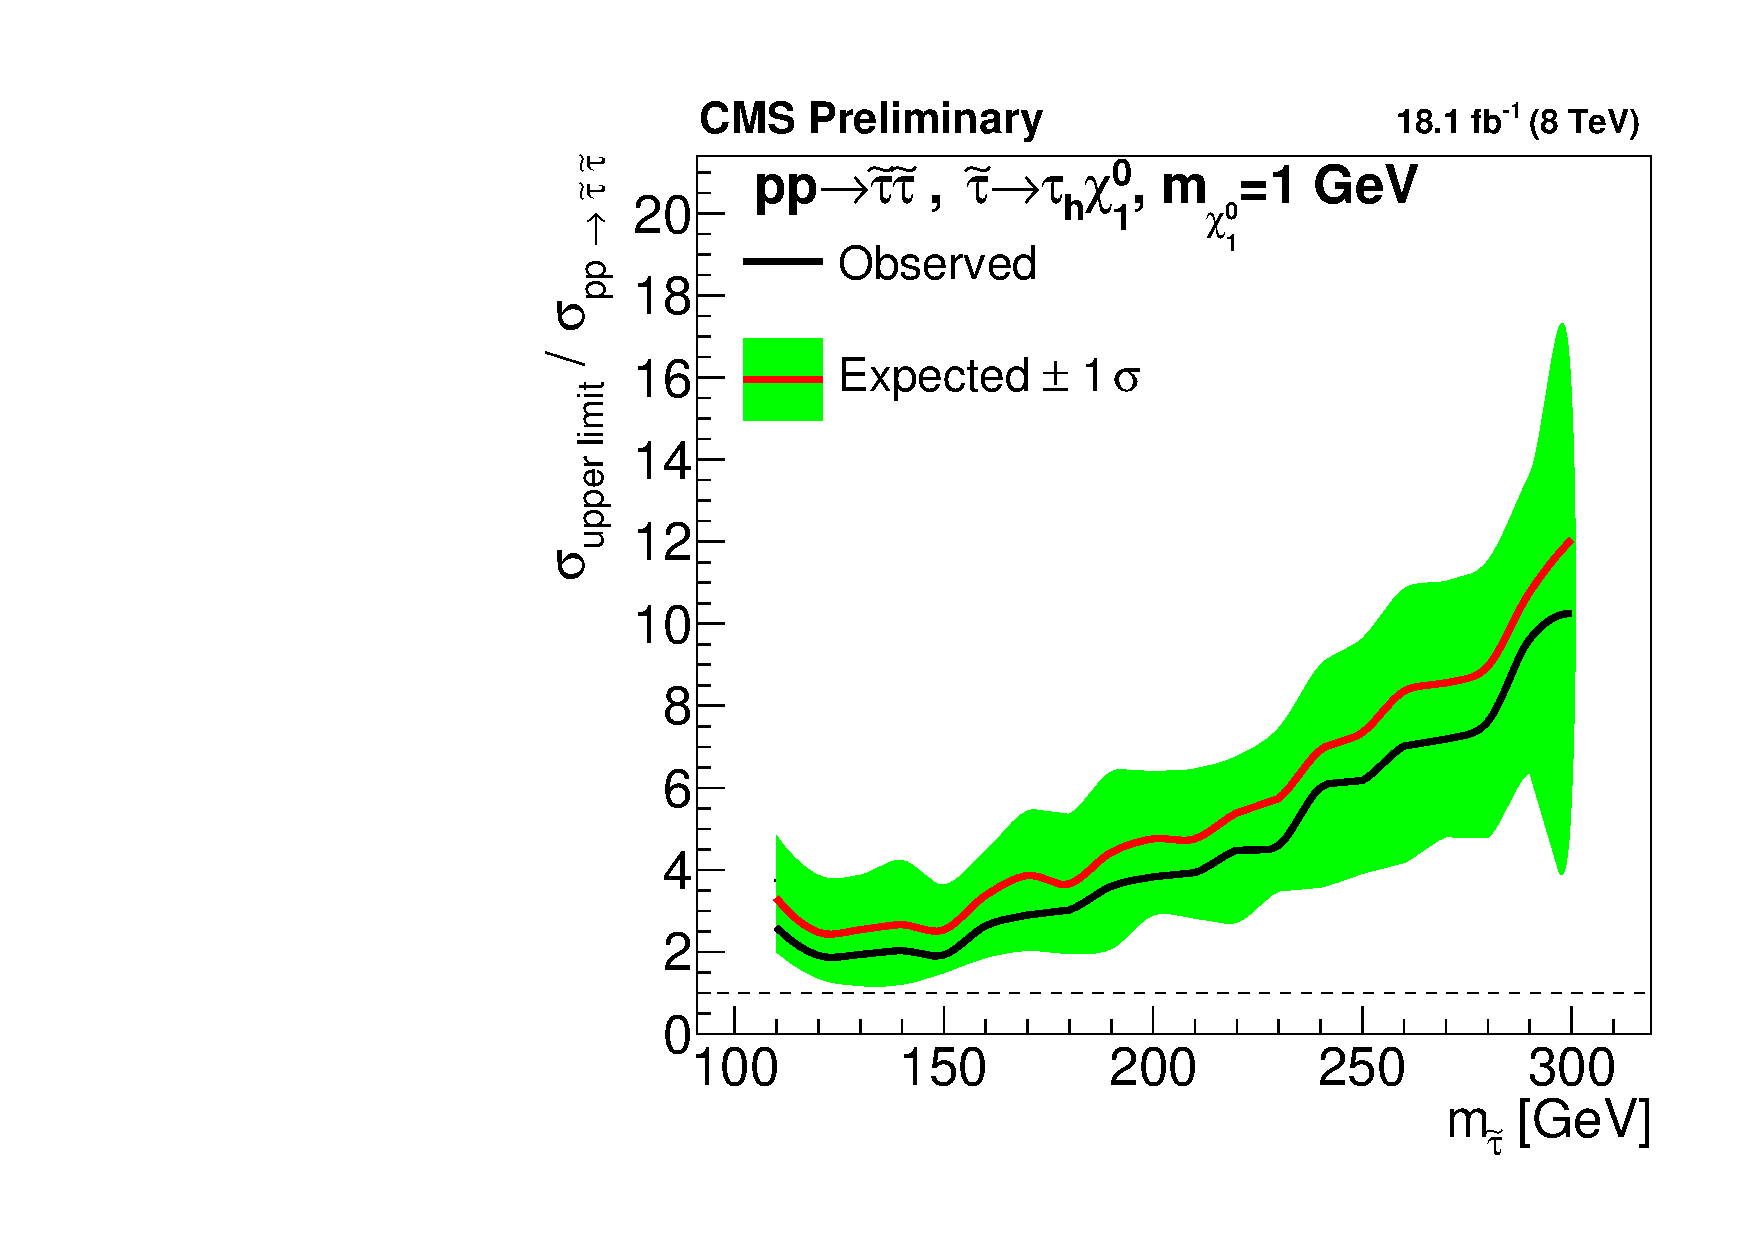
\includegraphics[width=0.5\textwidth,keepaspectratio=true]{StatisticsFig/ExclusionSTauSTauLsp1.pdf}
\caption{The exclusion power of the \tauTau channels in $\tilde{\tau}\tilde{\tau}$ production.}
\label{fig:limit_stau_stau}
\end{figure}
\end{linenomath}
 no point is excluded and $95\%$ upper limit is set on the cross section. Adding two $\ell\Tau$ channels does not improve the results.
Figure ~\ref{fig:limit_stau_stau} represents the ratio of the 
obtained upper limit on the cross section and the cross section expected from SUSY vs. the mass of the $\tilde{\tau}$ particle, when \PSGczDo mass is $1 GeV$.
The observed ratio is within one standard deviation of  the expected ratio. In the best point,  the upper limit is as large as two times of the theoretical 
cross section. 

%{\bf (You need to spend one sentence to explain what method you are using to set limits.  I assume
%  it is CLs, but because I am not sure what you actually did I did not write
%  it down.  Also, you
%  need to specify whether this is 95\% CL or 90\% CL or whatever).}
%{\bf (The description of the simplified model is insufficient.  Surely the cross-section and branching
%  ratios depends on the stau mass and/or the sneutrino mass?  It must also make a difference whether
%  the stau/sneutrino are on- or off-shell and what their masses are as far as the acceptance
%  is concerned.
%  Also in Figure 1 left there are two distinct
%  decay chains.  What BR are you assuming for the two chains)}
%{\bf The caption for the figure is incorrect..it says expected but there is also observed.  The boundaries
%  of the plot (diagonal lines) need to be explained.)}




